%% LaTeX2e class for student theses
%% sections/evaluation.tex
%% 
%% Karlsruhe Institute of Technology
%% Institute for Program Structures and Data Organization
%% Chair for Software Design and Quality (SDQ)
%%
%% Dr.-Ing. Erik Burger
%% burger@kit.edu
%%
%% Version 1.3.2, 2017-08-01

\chapter{Evaluation}
\label{ch:Evaluation}

In this section, we introduce the evaluation of our approach. We divided our evaluation into levels. In the first level, we evaluate the adaptive instrumentation. In the second level, we evaluate the monitoring information that we created to make sure that we’ve created the right monitoring information. In the third level, we evaluate our approach in term o reducing the monitoring overhead. \\
In the following we defined the goals (G) and research questions (Q) for our evaluation:\\

G1: Adaptive Instrumentation\\
  \quad Q1.1: Is our instrumentation of the source code incremental?\\
	  \qquad M1.1.1: difference between the probes in the instrumentation model and the probes logged in the        
	                monitoring information. \\
  \quad Q1.2: did we generate the right monitoring information?\\
	    \qquad M1.2.1: Number of acceptances of our monitoring information from performance model parameters  
	                         estimation approach.\\
G2: Adaptive Monitoring\\
   \hspace{10mm} Q2.1: How much monitoring overhead could we reduce?\\
        \hspace{20mm} M2.1.1: number of generated probes.\\


\section{Case Study}
\label{sec:Case Study}
In order to evaluate our approach, we performed a case study that is represented by the component diagram in Figure \ref{fig:case_study}. We created two Java interfaces and we implemented them. The first interface \textit{ISearchingAlgo} contains two functions. The service \textit{sequentianSearch}, which receives an Array of integers and a value of type integer, it returns True if the given value exists in the given array. This service is based on the sequential searching algorithm. The second service \textit{binarySearch} perform receives also an Array of integers and an integer value, it must then tell us if the given could be found in the given array. The service \textit{binarySearch} is implemented based on the binary searching algorithm. The binary searching algorithm is more efficient then the sequential searching algorithm, we choose these algorithms to provide the possibility of having different response times and service calls parameters. 

The second interface \textit{GuiSearchingAlgo} provides also two services and requires services from the interface \textit{ISearchingAlgo}. The service \textit{guiSeuentialSearch} receives two arrays of integers, the first array represents the array in which we want to perform the searching, the second array represent the values we want to search for. This service iterates over the  array of values that we want to search for and calls the service \textit{sequentialSeach} from the interface \textit{ISearchingAlgo}, which tells if the current searched value could be found. Figure 2 shows the corresponding SEFF of the \textit{guiSequentialSearch} service. The service \textit{guiBinarySearch} in the interface \textit{GuiSearchingAlgo} does the same thing as the service \textit{guiSequentialSearch} but it calls the service \textit{binarySearch} instead of \textit{sequentialSeach} service. 

\begin{figure}[h]
\centering
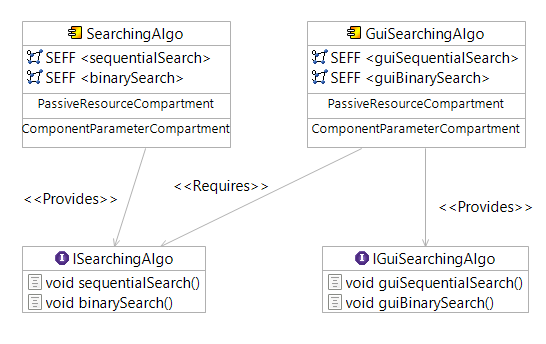
\includegraphics[width=0.9\textwidth]{figures/case_study}
\caption{Component diagram of our case study}
\label{fig:case_study}
\end{figure}



